% Copyright (c) 2026 Selina Cheggour. Tous droits réservés. Voir le fichier LICENSE.
% Partie 6 (fin de la chaîne principale), partie 7 (chaîne de comparaison), partie 8 (ce qui sort de Kaggle).

\bandeaupartie{I. Partie 6 : exporter, et le tableau de bord}{Des chiffres qui sortent, des textes qui restent : la fin de la chaîne principale.}

\section{Partie 6 : exporter les résultats pour le tableau de bord}

\begin{center}
\begin{tikzpicture}[
  col/.style={draw=#1, fill=#1!8, rounded corners=6pt, text width=4.6cm, align=left, font=\footnotesize, inner sep=7pt, minimum height=4.3cm},
  t/.style={font=\bfseries\small, color=#1}]
\node[col=accentblue] (a) {\textbf{\texttt{resultats.js}} \hfill{\color{accentblue}\faCheckCircle}\\[3pt]
comptes par période, langue, segment, marque\\ problèmes : taille, statut, langues\\ cases anormales et alertes\\ une position 3D par plainte (langue, période, problème)\\[3pt]\textit{les problèmes sont numérotés sur la base réelle}};
\node[col=sectioncolor, right=0.35cm of a] (b) {\textbf{\texttt{comparaison.js}} \hfill{\color{sectioncolor}\faCheckCircle}\\[3pt]
pour chaque modèle : temps, mémoire, paramètres, nombre de problèmes, stabilité, alertes\\[3pt]\textit{(deuxième grande partie)}};
\node[col=slate, right=0.35cm of b] (c) {\textbf{ne sortent jamais} \hfill{\color{slate}\faTimesCircle}\\[3pt]
les verbatims\\ les numéros de cas\\ les vecteurs \texttt{plongements\_*.npy}\\[3pt]\textit{et sur la base réelle, \texttt{noms\_problemes.js} reste pour la seule personne habilitée}};
\end{tikzpicture}
\end{center}

\begin{stepbox}[title={6\quad Une écriture fermée par défaut}]
Avant d'écrire, \texttt{ecrire\_export} arrondit tous les nombres à 4 décimales, puis cherche chaque numéro
de cas et chaque début de verbatim dans le texte de l'export. \textbf{S'il en trouve un, le fichier n'est pas
écrit} : la cellule affiche seulement le nom des champs en cause, jamais leur valeur.
\doisvoir{aucun numéro de cas ni verbatim dans l'export, le fichier du tableau de bord écrit, une position 3D par plainte.}
\image{un portique d'aéroport : la valise ne passe que si rien d'interdit n'est dedans, et l'agent dit \og poche de gauche \fg{} sans vider la valise devant tout le monde.}
\end{stepbox}

\begin{enfant}
\textbf{Pourquoi arrondir ?} Un nombre écrit avec 17 chiffres, comme \texttt{0.07199999690055847},
finit par contenir par hasard une suite de 7 chiffres identique à un numéro de cas. Arrondi à
\texttt{0.072}, il ne le peut plus.
\end{enfant}

%%%%%%%%%%%%%%%%%%%%%%%%%%%%%%%%%%%%%%%%%%%%%%%%%%%%%%%%%%%%%%%%%%%%%%%%%%%%%%%%%%%%%%%%%%%%%%%%%%%%%%%%
\section{Le tableau de bord}

Une page HTML qui fonctionne \textbf{sans internet} : on pose \texttt{resultats.js} et
\texttt{comparaison.js} à côté de \texttt{tableau\_de\_bord.html} et on l'ouvre. Chaque graphique a un
bouton {\color{accentblue}\textbf{\textit{i}}} qui l'explique simplement.

\illus[0.98\linewidth]{tdb_1_galaxie.png}{La galaxie des plaintes (base fictive) : chaque point lumineux est une plainte, chaque pastille un problème.}

\begin{lire}
\textbf{Comment lire la galaxie.} Deux points proches racontent à peu près la même chose, même dans deux
langues différentes. Un amas d'une même couleur est un problème trouvé sans qu'on dise à la méthode quoi
chercher. On fait tourner à la souris ; la liste de droite donne le numéro, les mots, et un badge
\og alerte \fg, \og saison \fg{} ou \og campagne \fg.
\end{lire}

\begin{tcbraster}[raster columns=2, raster column skip=8pt, raster every box/.style={unbreakable, colback=white, colframe=palblue, boxrule=0.6pt, arc=4pt, left=3pt, right=3pt, top=3pt, bottom=3pt}]
\begin{tcolorbox}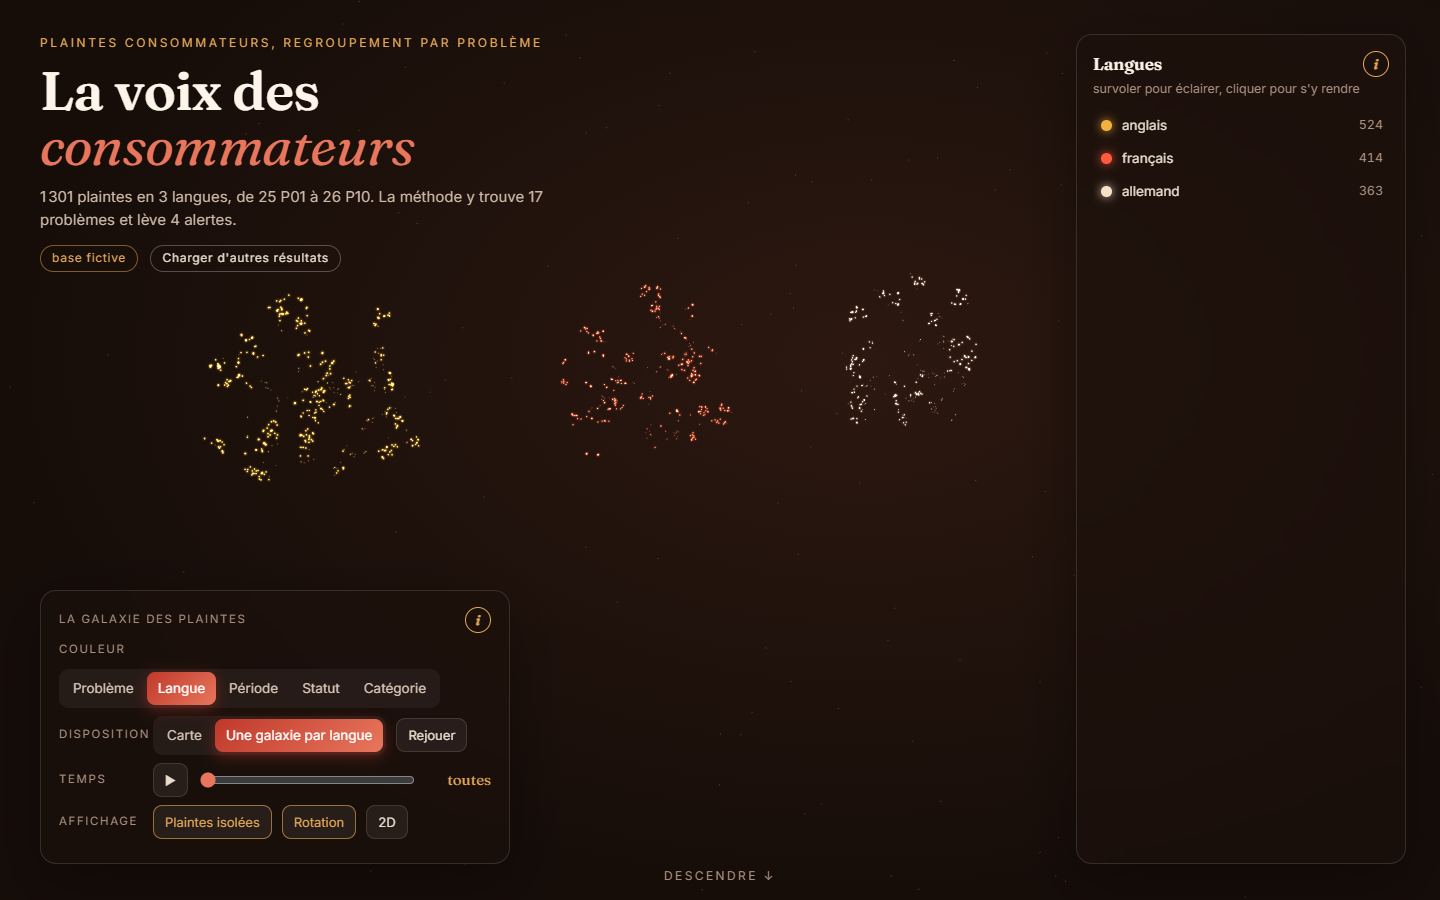
\includegraphics[width=\linewidth]{tdb_3_galaxie_par_langue.png}\\[2pt]{\footnotesize\textbf{Une galaxie par langue} : les mêmes amas reviennent dans chaque langue, donc les problèmes traversent les langues.}\end{tcolorbox}
\begin{tcolorbox}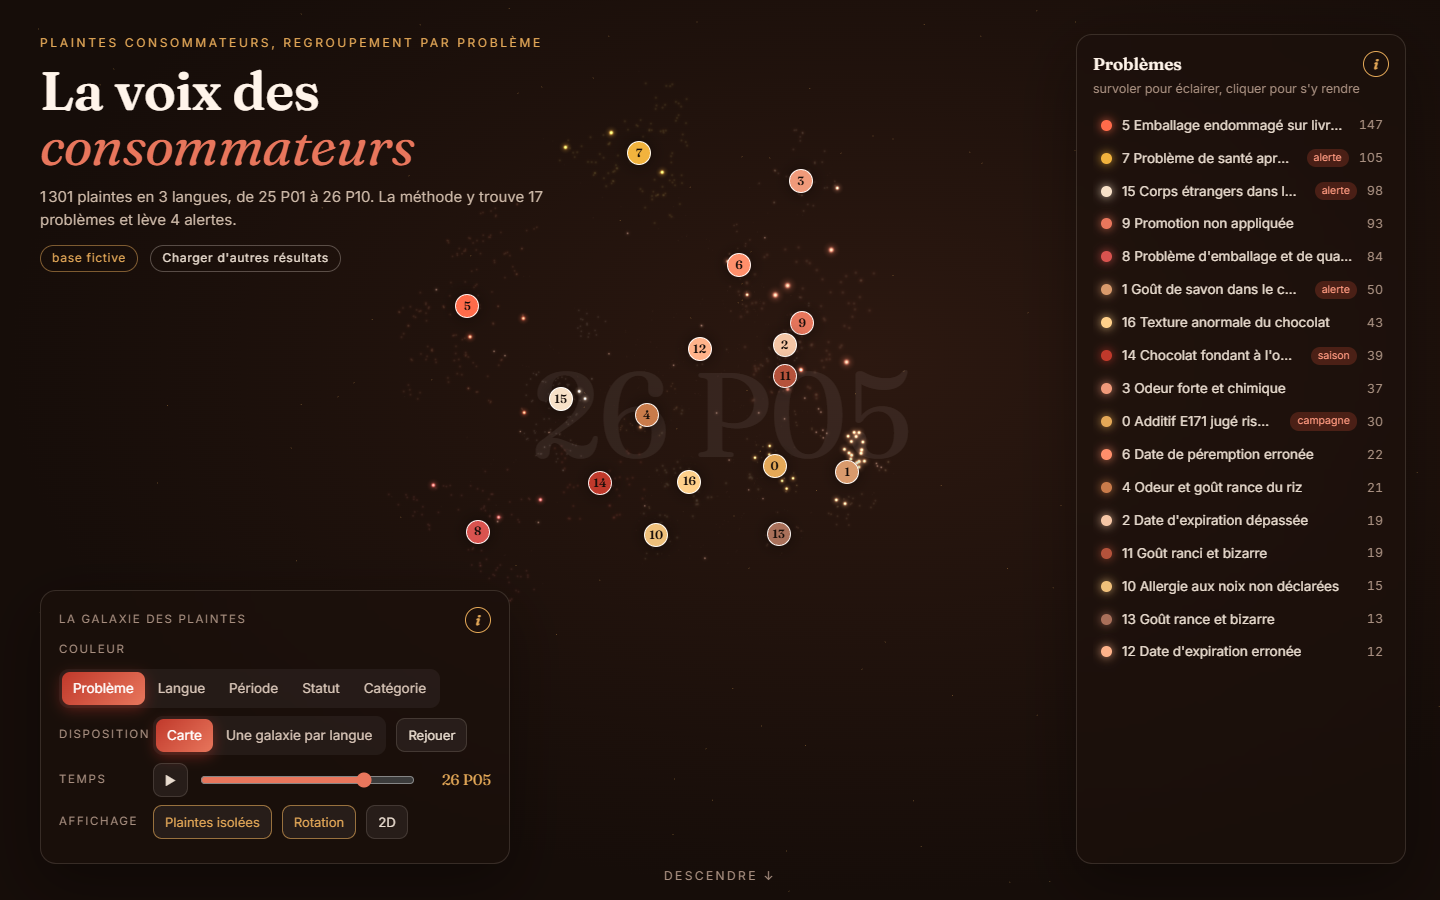
\includegraphics[width=\linewidth]{tdb_4_galaxie_periode.png}\\[2pt]{\footnotesize\textbf{Le temps} : le bouton \faPlay{} n'allume que les plaintes d'une période ; un amas qui s'allume d'un coup est un problème qui surgit.}\end{tcolorbox}
\begin{tcolorbox}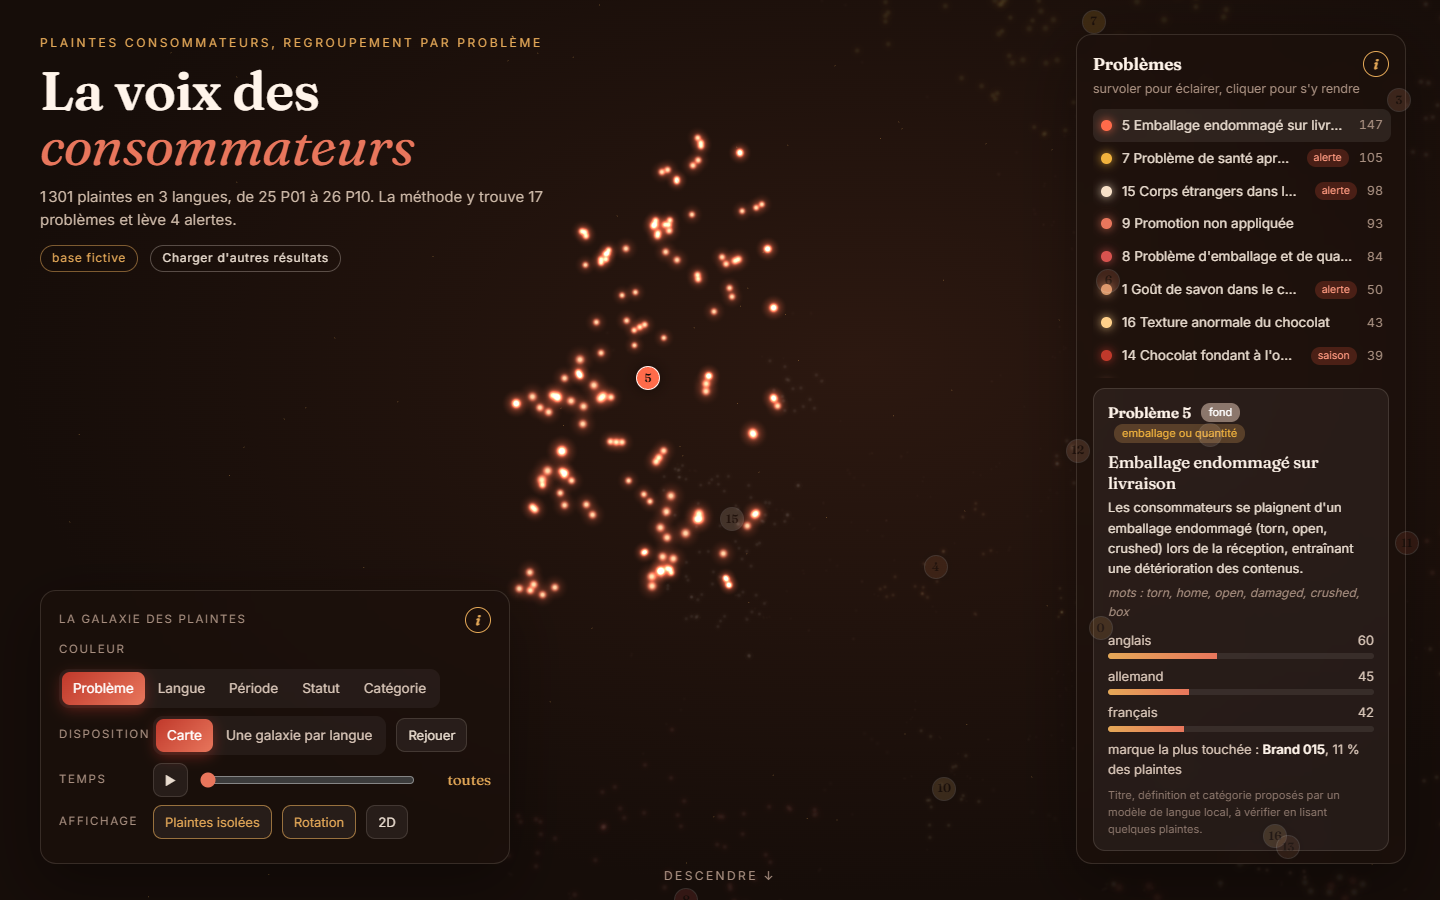
\includegraphics[width=\linewidth]{tdb_5_galaxie_focus.png}\\[2pt]{\footnotesize\textbf{Un clic sur un problème} : la caméra vole jusqu'à lui et sa fiche s'affiche (langues, marque la plus touchée, statut).}\end{tcolorbox}
\begin{tcolorbox}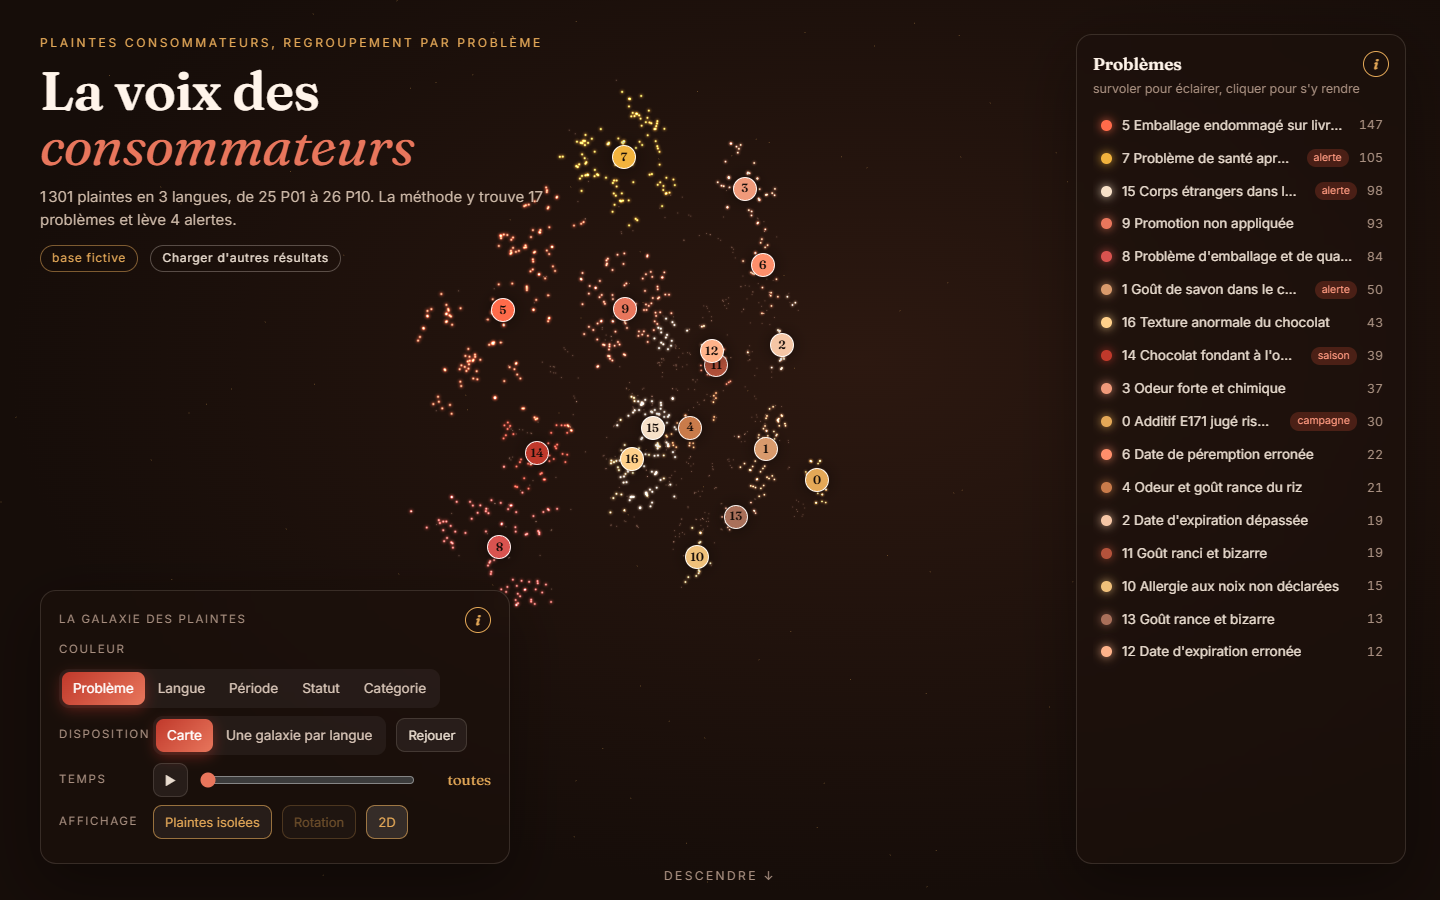
\includegraphics[width=\linewidth]{tdb_14_galaxie_2d.png}\\[2pt]{\footnotesize\textbf{Le bouton 2D} aplatit la galaxie pour la regarder de face.}\end{tcolorbox}
\begin{tcolorbox}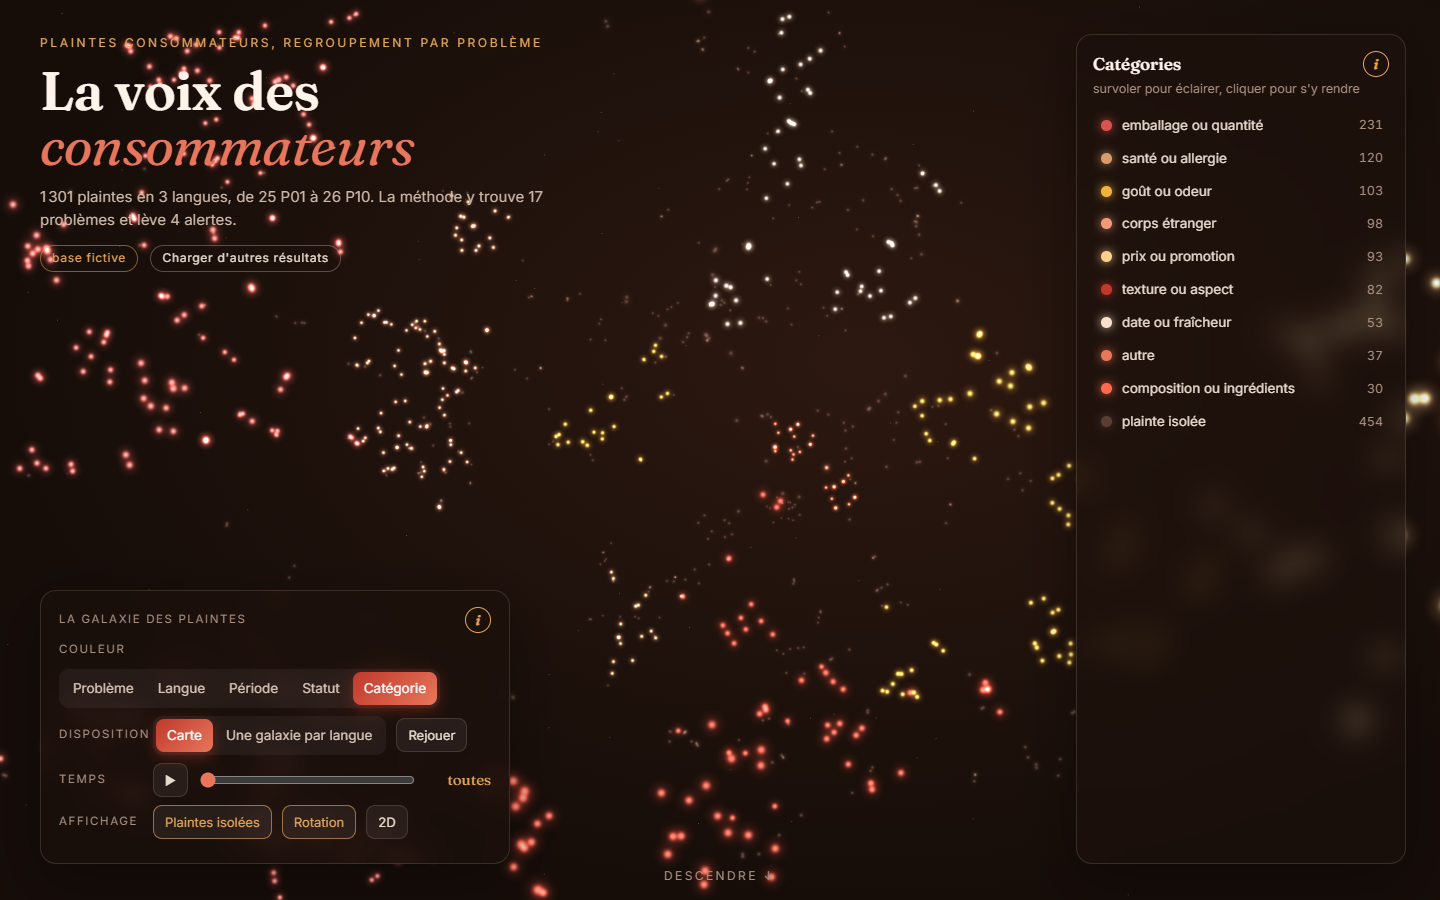
\includegraphics[width=\linewidth]{tdb_categorie_demo.png}\\[2pt]{\footnotesize\textbf{Le mode Catégorie} (base fictive) : chaque plainte prend la couleur de la famille de son problème, proposée par le modèle de langue local.}\end{tcolorbox}
\begin{tcolorbox}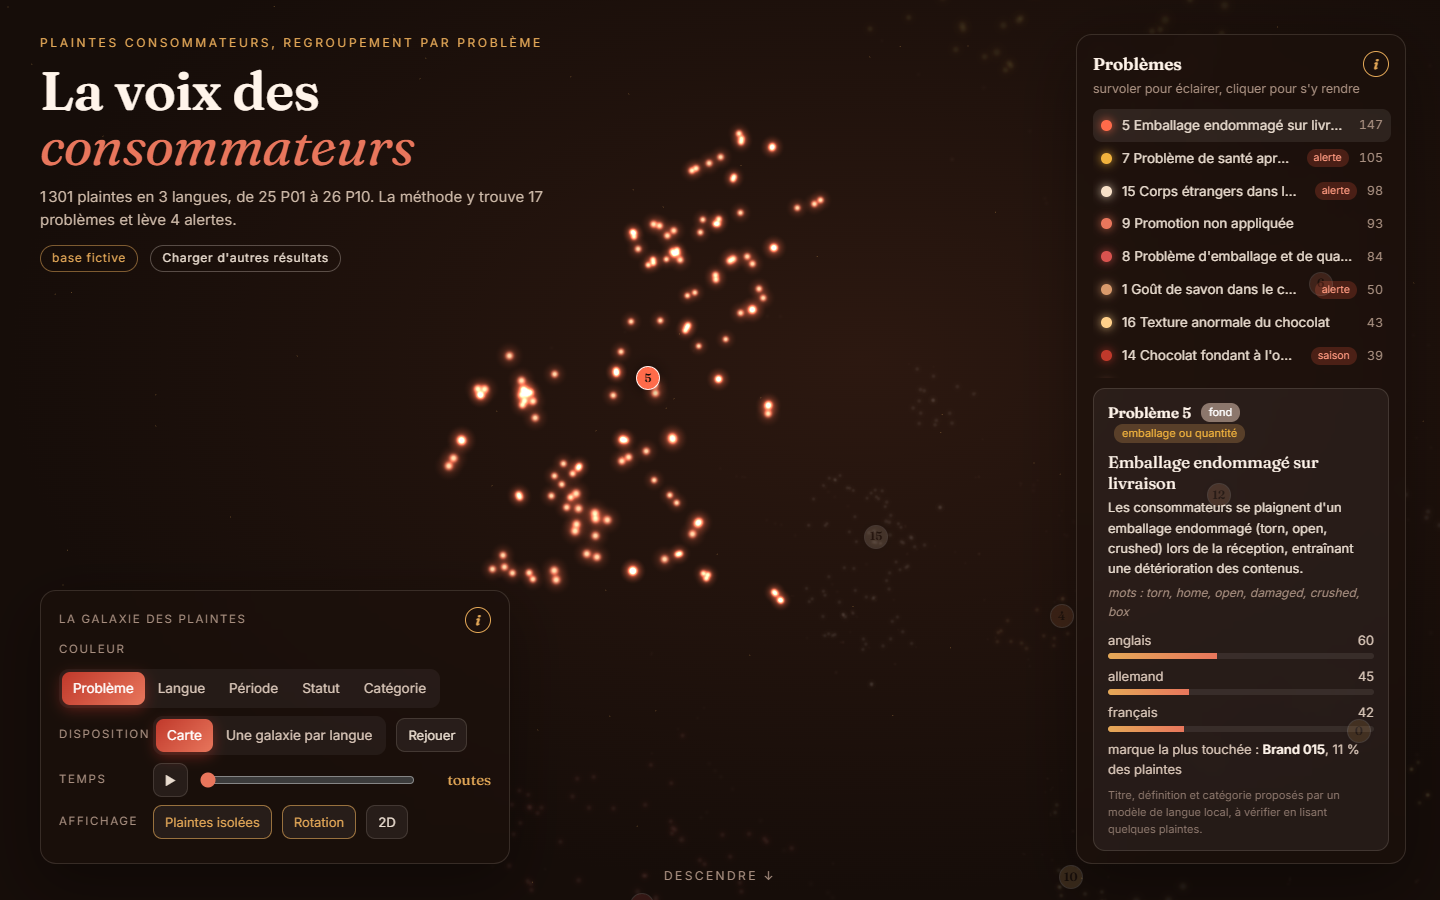
\includegraphics[width=\linewidth]{tdb_fiche_demo.png}\\[2pt]{\footnotesize\textbf{La fiche d'un problème} (base fictive) : titre, définition et catégorie proposés par le modèle de langue local, puis mots, langues, marque.}\end{tcolorbox}
\end{tcbraster}

\illus[0.98\linewidth]{tdb_8_relief.png}{Le relief des excès : chaque tour est une case problème $\times$ période.}

\begin{lire}
\textbf{Comment lire le relief.} La hauteur et la couleur disent combien de plaintes il y a eu par
rapport à ce qu'on attendait. Un problème normal a des tours plates ; une ou deux tours qui jaillissent
sur une ligne signalent un incident, une saison ou une campagne. Les tours rouge vif sont les alertes.
Le bouton \og À plat \fg{} montre la même chose en carte de chaleur.
\end{lire}

\illus[0.98\linewidth]{tdb_9_alertes.png}{Les cartes d'alerte, puis ce qui n'est pas un incident (saison, campagne).}

\begin{lire}
\textbf{Comment lire une carte d'alerte.} Le grand nombre : les plaintes de cette marque, pour ce
problème, à cette période ; à côté, combien on en attendait, et le rapport (\og $\times 16$ \fg{} : seize
fois plus). La phrase dit quelle part du pic porte la marque et quelle est la chance que ce soit le
hasard. Les petites barres reprennent la figure 5 du notebook.
\end{lire}

\begin{tcbraster}[raster columns=2, raster column skip=8pt, raster every box/.style={unbreakable, colback=white, colframe=palblue, boxrule=0.6pt, arc=4pt, left=3pt, right=3pt, top=3pt, bottom=3pt}]
\begin{tcolorbox}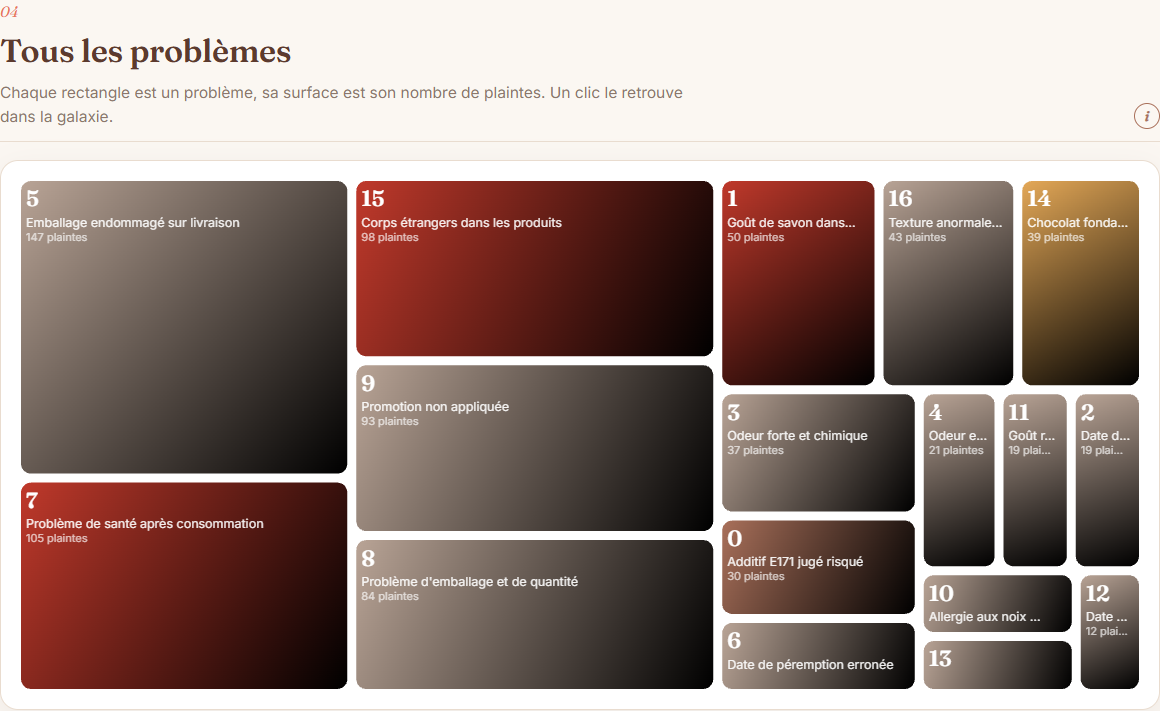
\includegraphics[width=\linewidth]{tdb_10_problemes.png}\\[2pt]{\footnotesize\textbf{La mosaïque} : un rectangle par problème, sa surface est son nombre de plaintes, sa couleur son statut. Un clic le retrouve dans la galaxie.}\end{tcolorbox}
\begin{tcolorbox}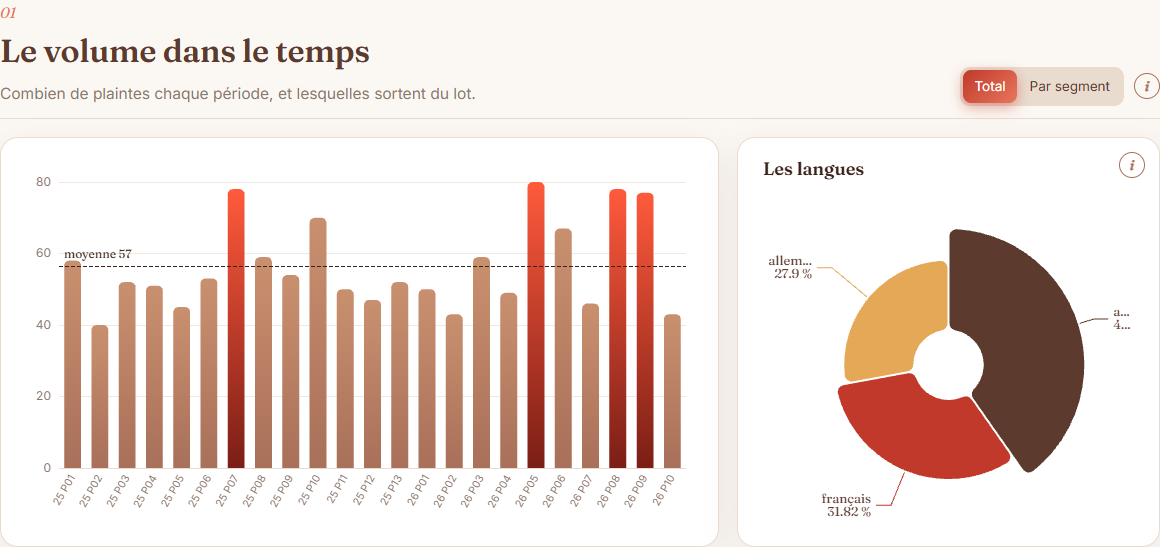
\includegraphics[width=\linewidth]{tdb_7_volume.png}\\[2pt]{\footnotesize\textbf{Le volume} par période, total ou par segment, avec les langues à côté.}\end{tcolorbox}
\begin{tcolorbox}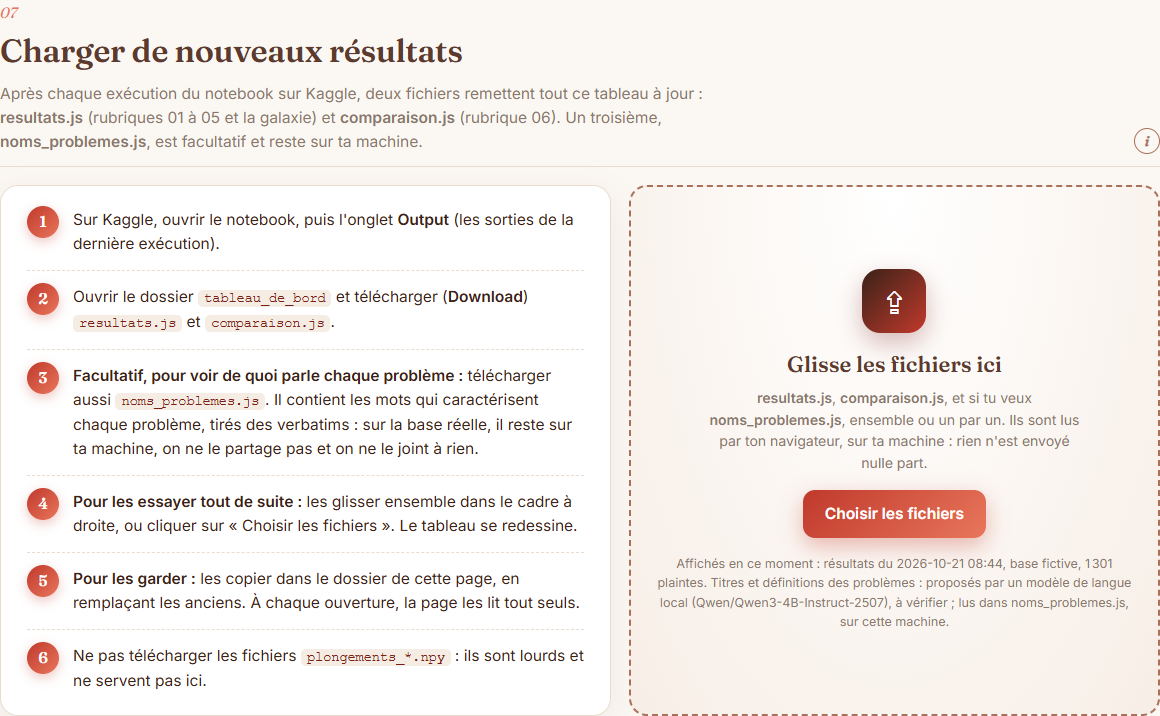
\includegraphics[width=\linewidth]{tdb_13_charger.png}\\[2pt]{\footnotesize\textbf{Charger de nouveaux résultats} : glisser les fichiers sur la page, ou les copier à côté d'elle.}\end{tcolorbox}
\end{tcbraster}

\illus[0.8\linewidth]{tdb_12_aide.png}{Le bouton \textit{i} : chaque graphique expliqué en quelques lignes.}

\bandeaupartie{II. La chaîne de comparaison}{La chaîne principale marche : on la rejoue avec huit outils, et on compare.}

\section{Avant de comparer : la chaîne principale est-elle validée ?}

\begin{stepbox}[title={7.0\quad Le bilan de la chaîne principale}]
La cellule 7.0 compte les vérifications \texttt{[OK]} de la chaîne principale, liste celles \texttt{[À revoir]}
et contrôle que \texttt{resultats.js} est écrit. \textbf{Lis chaque ligne \texttt{[À revoir]}} : ce n'est pas
forcément une erreur (une base sans incident ne lève aucune alerte), mais tu dois savoir l'expliquer.
\doisvoir{le nombre de vérifications réussies, la liste de celles à revoir, et \texttt{[OK]} pour \og la chaîne principale a écrit resultats.js \fg.}
\image{on goûte le plat avant d'acheter d'autres casseroles.}
\end{stepbox}

\begin{piege}
\textbf{Ne lance pas la comparaison sur une chaîne qui ne marche pas.} Si \texttt{resultats.js} n'est pas
écrit, reviens aux parties 0 à 6 : comparer huit outils sur une chaîne cassée ne dit rien de ces outils.
\end{piege}

\section{Partie 7 : comparer les outils}

La chaîne principale reste la même ; seule change la façon de transformer une plainte en vecteur.
Huit représentations, du comptage de mots à un transformer de 4 milliards de paramètres. Aucune
n'écrit de texte, et toutes tournent dans le notebook.

\begin{center}
\small
\renewcommand{\arraystretch}{1.22}
\rowcolors{2}{notebg}{white}
\begin{tabular}{@{}lllll@{}}
\rowcolor{titlebg}\color{white}\textbf{représentation} & \color{white}\textbf{origine} & \color{white}\textbf{type} & \color{white}\textbf{paramètres} & \color{white}\textbf{licence} \\
TF-IDF + SVD (100 dim.) & {\color{slate}\faFont}\ aucun créateur & comptage de mots & aucun & \\
MiniLM-L12 multilingue & \logo{sbert_logo}\logo{microsoft_logo} SBERT, Microsoft & transformer & 118 M & Apache 2.0 \\
e5-small multilingue & \logo{microsoft_logo} Microsoft & transformer & 118 M & MIT \\
e5-base multilingue & \logo{microsoft_logo} Microsoft & transformer & 278 M & MIT \\
e5-large multilingue & \logo{microsoft_logo} Microsoft & transformer & 560 M & MIT \\
BGE-M3 & \logo{baai_logo} BAAI & transformer & 568 M & MIT \\
\textbf{Qwen3-Embedding-0.6B} & \logo{qwen_logo} Alibaba (Qwen) & dérivé d'un LLM & 0,6 G & Apache 2.0 \\
Qwen3-Embedding-4B & \logo{qwen_logo} Alibaba (Qwen) & dérivé d'un LLM & 4 G & Apache 2.0 \\
\end{tabular}
\end{center}

% Copyright (c) 2026 Selina Cheggour. Tous droits réservés. Voir le fichier LICENSE.
% Tableau comparatif des modèles de plongement de la partie 7.
\subsection*{Tableau comparatif des modèles de plongement}

Les sept transformers de la partie~7 vont du modèle ultra-léger au modèle de plongement dérivé d'un LLM.
Les chiffres sont ceux des versions \textbf{multilingues} utilisées dans le notebook ; les versions
anglaises de MiniLM-L12 et de e5 sont plus petites (33, 110 et 335 M de paramètres).

\begin{center}
\scriptsize
\renewcommand{\arraystretch}{1.3}
\setlength{\tabcolsep}{2.5pt}
\rowcolors{2}{notebg}{white}
\begin{tabular}{@{}>{\raggedright\arraybackslash}p{2.1cm}>{\raggedright\arraybackslash}p{1.75cm}>{\raggedleft\arraybackslash}p{0.92cm}>{\raggedleft\arraybackslash}p{1.45cm}>{\raggedleft\arraybackslash}p{0.95cm}>{\raggedright\arraybackslash}p{4.18cm}>{\raggedright\arraybackslash}p{3.85cm}@{}}
\rowcolor{titlebg}\color{white}\textbf{modèle} & \color{white}\textbf{créateur} & \color{white}\textbf{param.} &
\color{white}\textbf{dim.} & \color{white}\textbf{jetons max} & \color{white}\textbf{points forts} &
\color{white}\textbf{usage idéal} \\
MiniLM-L12 multilingue & \logo{microsoft_logo}\logo{sbert_logo}\newline Microsoft, adapté par SBERT & 118 M & 384 & 128 &
Ultra-rapide, très peu gourmand, tourne sur processeur. &
Application légère, calcul en temps réel, petit budget d'infrastructure. \\
e5-small multilingue & \logo{microsoft_logo}\newline Microsoft & 118 M & 384 & 512 &
Rapide, bon rapport précision et vitesse, avec les préfixes \texttt{query:} et \texttt{passage:}. &
Prototype de RAG, moteur de recherche simple sur serveur léger. \\
e5-base multilingue & \logo{microsoft_logo}\newline Microsoft & 278 M & 768 & 512 &
Équilibré et polyvalent, meilleure finesse sémantique. &
Production standard, bon compromis entre coût et précision. \\
e5-large multilingue & \logo{microsoft_logo}\newline Microsoft & 560 M & 1\,024 & 512 &
Haute précision sémantique, capte bien les nuances. &
Recherche documentaire où la précision prime sur la vitesse. \\
BGE-M3 & \logo{baai_logo}\newline BAAI (Beijing Academy of AI) & 568 M & 1\,024 & 8\,192 &
Hybride, trois en un : dense, mots-clés (creux) et multi-vecteur (ColBERT). &
RAG sur documents longs qui demande à la fois le sens et les mots-clés exacts. \\
Qwen3-Embedding-0.6B (le modèle du TP) & \logo{qwen_logo}\newline Alibaba (Qwen) & 0,6 G & 1\,024 (32 à 1\,024, MRL) & 32\,768 &
Dérivé d'un LLM, sensible aux consignes, grande fenêtre de texte. &
RAG moderne sur textes longs, code, multilingue exigeant. \\
Qwen3-Embedding-4B & \logo{qwen_logo}\newline Alibaba (Qwen) & 4 G & 2\,560 (32 à 2\,560, MRL) & 32\,768 &
Parmi les meilleurs du classement MTEB multilingue à sa sortie (2025). &
Projet critique de très haute fidélité, avec une carte graphique dédiée. \\
\end{tabular}
\end{center}

\noindent{\footnotesize \textbf{param.} : nombre de paramètres. \textbf{dim.} : taille du vecteur produit.
\textbf{jetons max} : longueur maximale d'un texte, en jetons, au-delà de laquelle il est coupé.
\textbf{MRL} (\emph{Matryoshka Representation Learning}) : on peut ne garder que les premières coordonnées
du vecteur et perdre peu de qualité.\par}

\begin{notebox}[title={\faLightbulb\ Ce qu'il faut retenir pour choisir}]
\begin{itemize}[leftmargin=1.2em, itemsep=2pt]
\item Ultra-vitesse, sans carte graphique : MiniLM-L12 ou e5-small.
\item Un standard solide pour des textes courts ou moyens : e5-base ou e5-large.
\item Retrouver des mots-clés exacts (codes, références) dans des textes longs : BGE-M3.
\item Traiter de très longs documents (des PDF entiers) ou du code : Qwen3-Embedding (0.6B ou 4B).
\end{itemize}
Les plaintes du TP sont courtes et multilingues : c'est la mesure de la partie~7, pas ce tableau, qui
départage les modèles sur ces données.
\end{notebox}


\begin{stepbox}[title={7.1 à 7.4\quad Mesurer chaque modèle, à chaîne égale}]
\texttt{chaine(E)} reprend centrage, réglage automatique (3.3), regroupement, fusion et alertes,
sans graphiques. Pour chaque modèle on mesure :
\begin{formulabox}
\textbf{le temps} : $t^{\mathrm{ch}}$, chargement du modèle (téléchargement compris la première fois),
et $t^{\mathrm{calc}}$, calcul des $N$ vecteurs ; d'où $\tau = 1\,000\, t^{\mathrm{calc}} / N$, les secondes
pour 1\,000 plaintes.\\[3pt]
\textbf{la mémoire} : le maximum occupé sur la carte graphique.\\[3pt]
\textbf{le coût} pour $N'$ plaintes, avec un tarif horaire $p$ de la carte :
\[
c(N') = \frac{t^{\mathrm{ch}} + \tau\, N' / 1\,000}{3\,600} \times p .
\]
Kaggle est gratuit : $c$ est ce que coûterait la même carte louée. On suppose que le calcul croît comme
le nombre de plaintes.\\[3pt]
\textbf{la qualité} : la stabilité (ARI entre trois tirages de 90 \% des plaintes), le nombre de
problèmes et les alertes.
\end{formulabox}
\doisvoir{au moins cinq représentations mesurées, le TF-IDF compris, des temps positifs ; le fichier \texttt{comparaison.js} écrit, sans numéro de cas ni verbatim.}
\end{stepbox}

\illus[0.95\linewidth]{ill_comparaison_ari.png}{Base fictive, deux exécutions : avec les réglages fixes de 3.1 et 3.2, puis avec le réglage automatique de 3.3.}

\begin{lire}
\textbf{Comment lire ce graphique.} Une ligne par modèle. Le point cacao est l'accord avec les groupes
cachés quand tous les modèles ont les réglages choisis pour le modèle du TP ; le point rouge, quand chaque
modèle reçoit son propre réglage automatique. À droite, le nombre de problèmes trouvés dans les deux cas.
Plus le point est à droite, plus les problèmes trouvés coïncident avec les groupes cachés.
\end{lire}

\begin{questionbox}
\textbf{\faComments\ À discuter en équipe.} Avec les réglages fixes, cinq modèles réunissent presque tout
en 2 problèmes. Que vaut alors leur rappel, et pourquoi ce chiffre est-il trompeur ? Avec le réglage
automatique, certains modèles gagnent beaucoup, et le modèle du TP perd un peu : que mesure exactement la
règle de choix, et qu'est-ce qu'elle ne mesure pas ?
\end{questionbox}

\illus[0.86\linewidth]{tdb_15_outils.png}{Rubrique 06 du tableau de bord sur la base fictive, première exécution (réglages fixes).}

\begin{lire}
\textbf{Comment lire la rubrique 06.} Le podium donne le modèle le plus juste, le transformer le plus
rapide et la place du modèle du TP. Dans \og Qualité contre vitesse \fg, chaque bulle est un modèle
(taille : son nombre de paramètres) ; les bons choix sont en haut à gauche. Le temps sépare chargement et
calcul ; le coût se recalcule quand on change le tarif ou le nombre de plaintes ; la mémoire montre la
limite de 16 Go d'une carte T4.
\end{lire}

%%%%%%%%%%%%%%%%%%%%%%%%%%%%%%%%%%%%%%%%%%%%%%%%%%%%%%%%%%%%%%%%%%%%%%%%%%%%%%%%%%%%%%%%%%%%%%%%%%%%%%%%
\section{Partie 8 : ce qui peut sortir de Kaggle}

\begin{center}
\begin{tikzpicture}[
  num/.style={circle,fill=accentblue,text=white,font=\bfseries\Large,minimum size=0.9cm},
  lab/.style={align=center,font=\small,text width=4.2cm},
  arr/.style={-{Stealth[length=3mm]},very thick,color=accentblue}]
\node[num] (n1) {1}; \node[num,right=4.2cm of n1] (n2) {2}; \node[num,right=4.2cm of n2] (n3) {3};
\node[lab,below=2pt of n1] {\textbf{Add Input} : le jeu de données \textbf{privé} de la base réelle};
\node[lab,below=2pt of n2] {cellule 0.1 : le nom du fichier est déjà écrit, rien à modifier};
\node[lab,below=2pt of n3] {tout exécuter : aucun verbatim ne s'affiche};
\draw[arr] (n1) -- (n2); \draw[arr] (n2) -- (n3);
\end{tikzpicture}
\end{center}

\begin{tcbraster}[raster columns=2, raster equal height, raster column skip=8pt]
\begin{card}{sectioncolor}{\faSignOut*\ Ce qui peut sortir de Kaggle}
\begin{itemize}[leftmargin=1.3em,itemsep=2pt]
\item[\faCheck] le rapport de lecture, les comptes par langue, marque, période
\item[\faCheck] le nombre et la taille des groupes, la stabilité
\item[\faCheck] les cases anormales (numéro du problème, marque, période, observé, attendu, $q$)
\item[\faCheck] \texttt{resultats.js} et \texttt{comparaison.js}
\end{itemize}
\end{card}
\begin{card}{slate}{\faBan\ Ce qui ne sort pas}
\begin{itemize}[leftmargin=1.3em,itemsep=2pt]
\item[\faTimes] les verbatims et les numéros de cas
\item[\faTimes] les vecteurs \texttt{plongements\_*.npy}
\item[\faTimes] les mots et définitions des problèmes, sauf accord écrit de l'entreprise
\item[\faTimes] les figures 3 à 5, dont les légendes sont faites de ces mots
\end{itemize}
\end{card}
\end{tcbraster}

\begin{piege}
\textbf{Sur de vraies plaintes, des réglages trouvés ailleurs ne tiennent pas forcément.} Les
vraies lettres sont plus longues, plus variées, et peuvent contenir une grosse campagne. C'est exactement
pour cela que l'exercice 3.3 choisit le réglage sur les données elles-mêmes, avec un plan B.
\end{piege}
